\documentclass[conference]{IEEEtran}
\IEEEoverridecommandlockouts

\usepackage{cite}
\usepackage{amsmath,amssymb,amsfonts}
\usepackage{algorithmic}
\usepackage{graphicx}
\usepackage{textcomp}
\usepackage{xcolor}
\usepackage{tabularx}
\def\BibTeX{{\rm B\kern-.05em{\sc i\kern-.025em b}\kern-.08em
    T\kern-.1667em\lower.7ex\hbox{E}\kern-.125emX}}
\begin{document}

\title{Metrics About Fault-Proneness In Object-Oriented Systems}

\author{\IEEEauthorblockN{Sabrina Böhm}
\IEEEauthorblockA{\textit{Universität Ulm} \\
Ulm, Germany \\
sabrina.boehm@uni-ulm.de}}

% Notizen:
% - Vortrag auf deutsch ~20min
% - 12 Seiten Inhalt ohne Refs
% - zwischen 8 und 25 Refs 
% 
% TODO - im abstract teasern auf welche metriken man genau eingeht
% TODO - mehr im Intro aus abstract wiederholen, mehr sagen warum Fehlerauswirkungen kritisch sind, Auswirkungen von fehlern wie im abstract tiefer
% TODO - im Intro auch schon zitieren wenn man muss, study such as [1], wenn man genaue Studien anspricht
% TODO - im Intro was mach ich jetzt genau im folgenden noch mehr sagen
% TODO - Research objective ganz am Ende ins Intro verschieben
% TODO - und research objective in research methodolgy wieder aufgreifen (wie hab ich die Metriken gefunden, wie bin ich vorgegangen um sie zu vergleichen)
% TODO - argumentieren warum ich die 2 metriken rausgepickt hab

\maketitle

\begin{abstract}
	Software quality is becoming increasingly important in modern times. Faulty or insufficient software can have severe consequences. For this reason, aspects such as qualitiy, security, reliability and maintainability must be considered at an early stage of the development process. Early detection of bugs or problems in the software prevents enormously high costs at the later times. In safety-critical areas, for example, the property of fault-proneness must be carefully considered. In order to include this aspect early in the development process, there are a number of metrics and methods that can estimate the fault prediction or reduce the fault-proneness of the software. By following certain rules and procedures, high costs and time can be saved for both developers and consumers.
	The goal of this work is to illustrate some of the widely used methods and design metrics that consider fault-proneness in object-oriented systems.
	
\end{abstract}

\section{Introduction}

In the field of software development there are some keywords like security, consistency or reliability that are indispensable today. Everyone wants the best and most intelligent software, but with increasing complexity the possibility of fault-proneness in the software increases. In the following, the aforementioned topic is examined under the programming language model of object orientation and metrics that can be considered, which is an important topic in research trends in software technology nowadays.
One might think that testing the software and the resulting errors is one of the last steps in the software development process, but this is a false assumption. The earlier the system is examined and tested for critical points, the more work will be saved in later, more cost-intensive development steps.

A software fault is defined as an anomalous condition or defect at the component, device, or subsystem level that can lead to a failure. Therefore an undesirable companion of developing, where the objective is to appear as little as possible.
Fault-proneness is an important external software quality attribute of interest to software developers and practitioners. The fault-proneness of an object-oriented class indicates the extent to which the class, given the metrics for that class, is fault-prone. Since it is difficult to measure the fault-proneness of software that is not yet in use, predictive models are applied to estimate the fault-proneness of software classes.

Several studies like "\textit{Fault-Proneness of Open Source Software: Exploring its Relations to Internal Software Quality and Maintenance Process}" \cite{kozlov2013fault} or "\textit{Empirical analysis for investigating the effect of object-oriented metrics on fault proneness: a replicated case study}" \cite{b2aggarwal2009empirical} have been carried out to determine which metrics are useful in capturing important quality attributes such as fault-proneness  and fault prediction, which are summarized in the following sections.
Furthermore the main research objective is the consolidation of some metrics and methods related to fault-proneness in the software development process.

This paper is organized as follows: Section \ref{content} deals with the content background of design metrics in object-oriented systems and the basic technologies about object orientation. In Section \ref{research} the research methodology is described. Afterwards the Section \ref{related} presents some studies and further literature that handle the concept of fault prediction and further analysis in that topic area. After the related work, it comes to the Section \ref{analysis}, that contains the analysis and summary of obejct-oriented design metrics and the results of some empirical studies that are concerned with fault-proneness and that used to support the software development process. After the investigation of the effects on these metrics, a discussion follows in Section \ref{discussion}, including the classification of the relevance in the software development process and the parties involved.Furthermore there are limitations and benefits of the considered metrics. Finally, the paper is concluded and gives an outlook in Section \ref{conclusion}.
\section{Content Background}\label{content}

%Um noch Inhalt zu gewinnen könntest du Object-Orientieted Programmierung erläutern und sagen zu was sie sich abgrenzt(Imperative Programmierung usw.)
%== als eigene Sektion wennn ich noch Platz brauch -> SUBSECTION!
In the following, we will consider fault-proneness as already mentioned, but from a restricted point of view, in an object-oriented context. Many software systems in use are based on object-oriented design. This means that data and program code are encapsulated in reusable objects. Everything is based on the communication of objects. For this purpose, classes, interfaces and methods, as well as attributes are declared and thus serve to represent states. This structure alone protects against fault-proneness, since the code is reusable and thus the programming effort is reduced \cite{fichman1993adoption}. Therefore, object orientation in itself offers advantages for maintainability and reusability \cite{lanza2002beyond}. Thus, fewer errors occur and the fault-proneness is reduced, too. 

In the object oriented context there are a few constructs like class, coupling, cohesion, inheritance, information hiding and polymorphism, which also influence the fault-proneness. Examples of languages that program object-oriented are C\#, C++ or Java.
%Wenn du dich hier auf die CK metriken beziehst ist es nicht knowledge sondern influence. Siehe CBO definition von CK metriken(Chidamber und Kernerer)
%zitate für metriken
One of the most common aspects incorporated into metrics is that of coupling, which refers to the degree of direct knowledge that one element has of another. For example subclass coupling describes the relationship between a child and its parent. The child is connected to its parent, but the parent is not connected to the child. 
%ich vermute mal du willst hier sagen das die parent class "einfluss" auf die Kinder hat und nicht anders herum. Schreib das er irgendwie so: .. therefore the parent class influences the inherited classes throguh the inherited methods .... -> umformulieren den satz
The degree of interconnection of the whole system is a key element in software development, i.e., it is important how big the effect of changing one attribute of one class has on all others and especially how many.
Therefore coupling plays a central role in the effects of software faults. It is defined as the degree of interdependence or the strength of relationship between software modules.
To give a short introduction in object orientation and the relation between its properties, it is shown in figure \ref{fig0}, that the general aspects as class, method and attribute depend on each other. Invoking methods and accessing attributes is the basic principle of communication of object-oriented software systems, which means that faults can occur here depending on the frequency of use of the methods or attributes.

\begin{figure}[htbp]
	\centerline{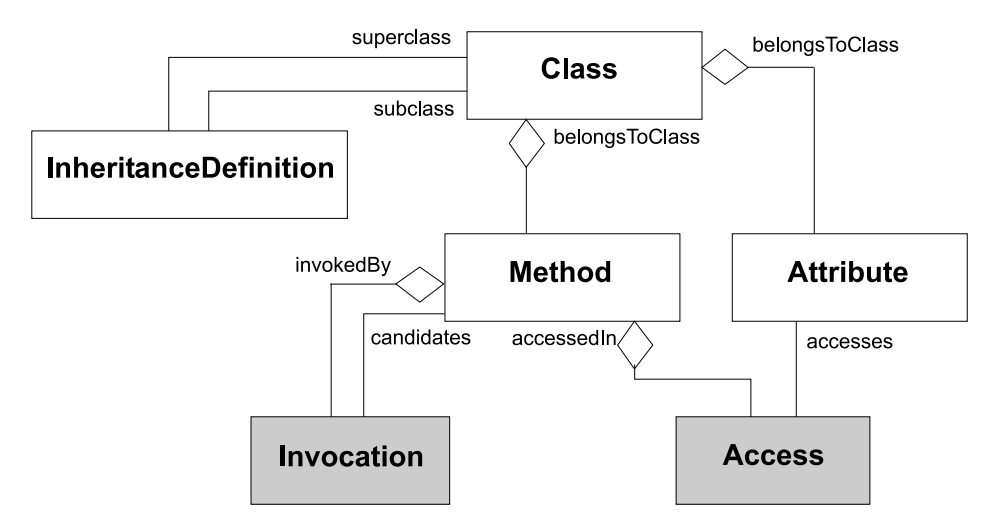
\includegraphics[width=0.5\textwidth]{pictures/oodesign.png}}
	\caption{A model for programming concepts with classes \cite{lanza2002beyond}.}
	\label{fig0}
\end{figure}

In how far the interaction of the individual components are connected with the fault-proneness metrics, this is described in the summary of metrics Section \ref{analysis} more near.%hier fehlt irgendwo ein wort

But why should a programmer actually pay attention to fault-proneness at all? The accurate prediction of where bugs are more likely to occur in the code can help manage efforts in testing, reduce costs, and improve the quality of the software. For different programming paradigms and programming constructs different rules apply which must be considered in relation to fault-proneness.  The restriction on object orientation is to facilitate the understanding. In addition many principles are contained, which are taken up in other programming concepts again. Thus some conclusions which are drawn here are also differently realizable and applicable to other software concepts.
%das ist motivation, hier nicht rein sondern nur fakten hier zur background work. Moti kommt in einleitung

In terms of fault-proneness, other quality characteristics that must not be forgotten also play a role like reliability, correctness, completeness, maintainability, as some are dependent on each other in terms of time. For example, software may not be reliable or correct if faults occur frequently that cause the software to become unusable.%das genauso eher motivation

When software errors are made, it is often not only tedious to find the programming error, but also expensive. In large systems that are used by many people every day, a small error can cost millions. A common misconception is that fault-proneness should only be considered at the end of the software development process. Especially at the beginning of the development you should build the software architecture in a way that it is less fault-prone. Changes in the architecture are always more expensive later. In addition, even before the programming itself begins, attention should be paid in the planning to various concepts and metrics, which are shown below.

%hier noch fault proneness erklären als eigene sektion maybe und fault und error etc.
\section{Research Methodology}\label{research}

First, this paper deals with research on the keywords "fault-proneness", "fault-proneness in object-oriented systems" and "fault prediction metrics". To get more literature on this topic, the keywords linked in the papers were used as further search. Among them are "object-orientation", "object-oriented design metrics" and "faulty classes". As first an overview was created in such a way, in order to be able to classify the term "fault-proneness" into the software development process. The top listed papers that were suggested in google scholar were either sorted out or read more closely by reading the abstract. If the abstract sounded interesting for the topic, then the introduction was read and the conclusion. In some papers, such as the research on metrics, the exact procedure and the analysis section were also read in detail. Two of the metrics were then chosen as a showcase model to illustrate fault-proneness in software systems. Further literature was researched for the content background to summarize the basic knowledge about object orientation and a simple understanding of objects, classes and methods.




\section{Related Work}\label{related}

To take a close look at fault-proneness in object oriented systems, basic object orientation knowledge is important, as explained in section \ref{content}. The paper "\textit{Beyond Language Independent Object-Oriented Metrics: Model Independent Metrics}" \cite{lanza2002beyond} deals not only with the concept of object orientation but also beyond languages and paradigms. The aspects of object orientation such as class, method and attribute can be found as shown in the following tables, which are subdivided into individual metrics. The model from figure \ref{fig0} serves as a template to understand the relationships between the individual metrics. 

In the following tables \ref{tab:classmetrics},\ref{tab:methodmetrics} and \ref{tab:attributesmetrics} the abbrevations and the associated metrics are listed. The used model and the metrics of the tables allow a multiple extension into different research directions. Thus, they fit the principle of object orientation and serve as a basic template to get into the basic structure of metrics. The advantages of this approach are the increased flexibility, i.e., new metamodels can be introduced from any context (for example, the financial world or databases), which provides a standard metric without the need to implement new metrics every time a new context is introduced \cite{lanza2002beyond}. Now, if you look at this system completely from an object orientation perspective, you can see that the basic programming concepts are translated into metrics. Each new method or variable crates more space to generate faults. The complexity of a class is depends, i.e., on the number of methods (NOM) or the number of attributes (NOA), that can be calculated with $NOA = NIV + NCV$, as shown in table \ref{tab:classmetrics}. An important metric about the methods of a class is the number of input parameters (NOP) or the number of access on attributes (NMAA), as you can see in figure \ref{tab:methodmetrics}. For the attribute metrics, the number of direct hits is of great importance, as can be found in figure \ref{tab:attributesmetrics}. 

\begin{table}
	\caption{Class metrics from the meta model.}~\label{tab:classmetrics}
	
	\setlength\tabcolsep{3pt}
	\renewcommand{\arraystretch}{1.4}% for the vertical padding
	\begin{tabularx}{\columnwidth}{ | c | p{7cm} | }
		\hline
		Abbrevation & Description \\ \hline\hline
		HNL & Number of classes in superclass chain of class \\ \hline
		NAM & Number of abstract methods \\ \hline
		NCV & Number of class variables \\ \hline
		NIA & Number of inherited attributes \\ \hline
		NIV & Number of instance variables \\ \hline
		NME & Number of methods extended, i.e., redefined in subclass by invoking the same method on a superclass \\ \hline	
		NMI & Number of methods inherited, i.e., defined in superclass and inherited unmodified by subclass\\ \hline
		NMO & Number of methods overridden, i.e., redefined compared to superclass\\ \hline
		NOA & Number of attributes $(NOA = NIV + NCV)$ \\ \hline
		NOC & Number of immediate subclasses of a class \\ \hline
		NOM & Number of methods\\ \hline
		PriA & Number of private attributes (equivalent for protected and public attributes)\\ \hline
		PriM & Number of private methods (equivalent for protected and public attributes)\\ \hline
		WLOC & Sum of all lines of codes over all methods \\ \hline
		WMSG & Sum of message sends in a class\\ \hline
		WNMAA & Number of all accesses on attributes\\ \hline
		WNOC & Number of all descendant classes\\ \hline
		WNOS & Sum of statements in all method bodies of class\\ \hline
		WNI & Number of invocations of all methods \\ \hline
	\end{tabularx}
\end{table}

\begin{table}
	\caption{Method metrics from the meta model.}~\label{tab:methodmetrics}
	
	\setlength\tabcolsep{3pt}
	\renewcommand{\arraystretch}{1.4}% for the vertical padding
	\begin{tabularx}{\columnwidth}{ | c | p{7cm} | }
		\hline
		Abbrevation & Description \\ \hline\hline
		LOC & Method lines of code \\ \hline
		NMA & Number of methods added, i.e., defined in subclass and not in superclass \\ \hline
		MSG & Number of method messages send \\ \hline
		NOP & Number of input parameters \\ \hline
		NI & Number of invocations of other methods within method body \\ \hline
		NMAA & Number of access on attributes \\ \hline
		NOS & Number of statements in method body \\ \hline
	\end{tabularx}
\end{table}

\begin{table}
	\caption{Attribute metrics from the meta model.}~\label{tab:attributesmetrics}
	
	\setlength\tabcolsep{3pt}
	\renewcommand{\arraystretch}{1.4}% for the vertical padding
	\begin{tabularx}{\columnwidth}{ | c | p{7cm} | }
		\hline
		Abbrevation & Description \\ \hline\hline
		AHNL & Class HNL in which attribute is defined \\ \hline
		NAA & Number of times directly accessed \\ \hline
	\end{tabularx}
\end{table}

Many metrics used in various studies are reflected in the tables.
The limitations of this approach are that not all object-oriented software metrics can be defined in terms of the language independent model, but these metrics serve as a basic overview. Certain metrics tend to be very specialized and are therefore difficult to define in a generic way. Another limitation of this basic concept is that for some metrics, there is it is not yet known how best to define them in a generic way, so the meta model does not include coupling metrics and cohesion metrics.

In another paper, a systematic literature review was reviewed that looked at 106 papers published between 1991 and 2011.
Object-oriented metrics (49\%) were used almost twice as often as traditional source code metrics (27\%) or process metrics (24\%). Object-oriented and process-oriented metrics were reported to be more successful in finding bugs compared to traditional size and complexity metrics \cite{b7radjenovic2013software}. The results of the literature review show that an inheritance and an export coupling metric are strongly associated with fault-proneness. Some evidence also suggests that there may be a small number of metrics that are strongly associated with fault-proneness, and that good predictive accuracy and quality estimation accuracy can be achieved with them.

Today's evidence suggests that most faults in software applications are found in a small percentage of software components \cite{b10el2001prediction}. This means that if these faulty software components can be identified early in the lifecycle of the development project, mitigation measures can be taken, such as redesign or refactoring. For object-oriented applications, predictive models using design metrics can be used to identify faulty classes early on \cite{b10el2001prediction}. The next step is to look at related work based on the metrics just presented and expansions of those. 

In the "\textit{Fault-Proneness of Open Source Software: Exploring its Relations to
Internal Software Quality and Maintenance Process}" \cite{kozlov2013fault} study, it was investigated how the fault-proneness of open source software (OSS) can be explained in terms of internal quality attributes and metrics of the maintenance process. A total of 342 releases of these systems were studied and, as usual, software quality was considered as a set of internal and external quality attributes. A total of 76 internal quality attributes were measured and 23 maintenance process metrics were included in this study. The strengths of this study is the comparison of a few software technology trends like fault-proneness and maintainability, as well as the study itself. First the study considers a wide range of metrics than common studies. Furthermore more OOS systems were involved in order to get a better indication of the results. In addition they focused on the fault-proneness of modern Java-based systems and investigated them as an aggregated sample. The framework for assessing the maintenance process was adopted from their previous studies. The results of the factor analysis performed showed that the metrics studied can be interpreted in terms of two factors, one of which is the system size, as shown in Figure \ref{figSize}. Previous studies in this area are based only on relatively small sets of OSS systems and releases, despite the fact that OSS projects are very diverse and heterogeneous \cite{kozlov2013fault}. Conclusively, the results may not be generalizable due to their relatively limited nature. Here, larger systems were chosen and size was found to play an important aspect in fault-proneness. In many other studies only small software systems were considered and it is noticeable that many in their conclusion note that a limitation of their work is that the statements can only be applied to small sized systems \cite{kozlov2013fault, b7radjenovic2013software}.

\begin{figure}[htbp]
	\centerline{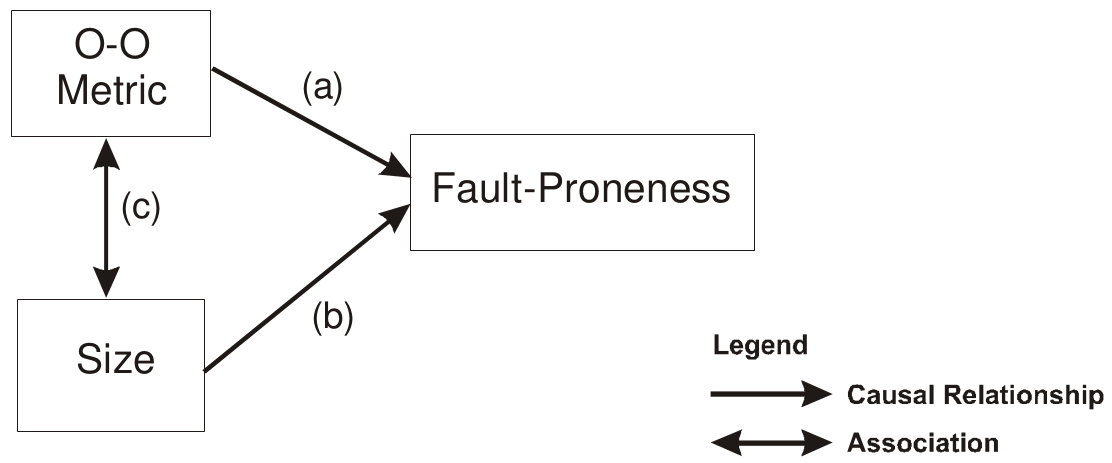
\includegraphics[width=0.45\textwidth]{pictures/faultyclasses2.png}}
	\caption{Path diagram illustrating the confounding effect of class size on the relationship between an object-oriented metric and fault-proneness \cite{b10el2001prediction}.}
	\label{figSize}
\end{figure}

Another study, also dealt with object-oriented design metrics for Java applications and construct a prediction model. It became clear that an export coupling metric exhibited the strongest association with fault-proneness, indicating a structural feature that may be symptomatic of a class with a high probability of latent faults \cite{b10el2001prediction}.

A theoretical basis for developing quantitative models that relate object-oriented metrics and external quality metrics is summarized in Figure \ref{figCoupling}. As already mentioned, one of the strongest association with fault-proneness was an export coupling metric in a study. This illustrates that there is a presumed relationship between object-oriented metrics and fault-proneness due to the effect on cognitive complexity \cite{b10el2001prediction}. Cognitive complexity can be defined as the mental load of the individuals who have to interact with the component, for example, the developers, testers, inspectors, and maintainers. 

\begin{figure}[htbp]
	\centerline{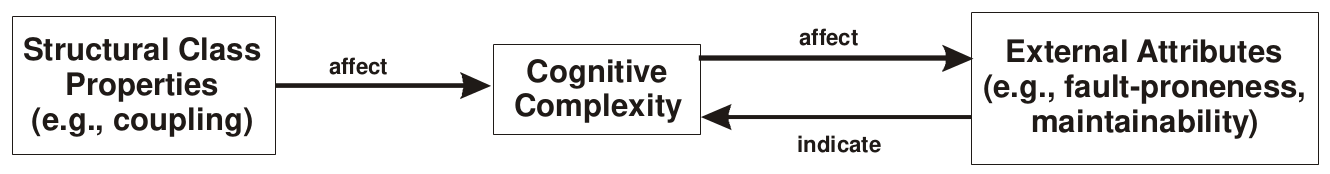
\includegraphics[width=0.5\textwidth]{pictures/faultyclasses1.png}}
	\caption{Theoretical basis for the development of object oriented product metrics \cite{b10el2001prediction}.}
	\label{figCoupling}
\end{figure}

Some studies also suggest that the depth of inheritance has an impact on the comprehensibility of object-oriented applications, and therefore would be expected to have a detrimental effect on fault-proneness \cite{b10el2001prediction}.
It was also found that inheritance leads to distributed class descriptions. That is, in this case, the complete description for a class can only be assembled by examining both the class itself and each of the superclasses of it.
Since different classes are described in different places in the code of a software program, also often distributed over several files, a programmer must turn to several places, in order to receive a complete description of a class. While this argument applies to software source code, it is not difficult to generalize it to design documents. Faults are therefore very distributed and usually cannot be found and fixed in a single place without making other changes.

Another study has considered a used set of ten software product metrics related to the following software attributes: the size of the software, coupling, cohesion, inheritance, and reuse \cite{yu2002predicting}. Some hypotheses regarding fault-proneness were empirically tested in a case study examining the client side of a large network service management system. The system under consideration is written in Java and consists of 123 classes. Validation was performed using two data analysis techniques: regression analysis and discriminant analysis.

Among other things, Class cohesion is a key attribute used to assess the design quality of a class and refers to the extent to which the methods and attributes of a class are related. Typically, classes contain special types of methods, such as constructors, destructors, and access methods, where each of these special methods has its own properties that can affect the measurement of class cohesion \cite{b4al2012impact}. Here we see again that the metrics can all be derived from the tables \ref{tab:classmetrics} and \ref{tab:methodmetrics} below.

Another paper empirically examines this impact of methods on cohesion measures. Twenty existing class cohesion metrics were used and Two types of special methods were considered, constructors and access methods. The empirical study applies the metrics, to five open source systems under four different scenarios, including first considering all special methods, second ignoring only constructors, third ignoring only access methods, and fourth ignoring all special methods.
The results of the empirical investigations show that the cohesion values for most of the considered metrics differ significantly in the four scenarios, but do not significantly affect the abilities of the metrics to predict faulty classes \cite{b4al2012impact}.

Based on this research, two more specific metrics have now been picked out, that try to support the software development process with their metrics. All of them work in their own way and in certain states of development. 
In order to provide guidance on how to proceed in the software process, some special metrics will be explained in detail now.


%A Validation of Object-Oriented Design Metrics as Quality Indicators ::: his paper presents the results of a study in which we empirically investigated the suite of object-oriented design metrics introduced in. More specifically, our goal is to assess these metrics as predictors of fault-prone classes and, therefore, determine whether they can be used as early quality indicators. This study is complementary to the work described in [30] where the same suite of metrics had been used to assess frequencies of maintenance changes to classes \cite{b11basili1996validation}.



%Assessing the Applicability of Fault-Proneness Models Across Object-Oriented Software Projects ::: Furthermore a number of papers have investigated the relationships between metrics of design and the metrics that detect faults in object oriented software. One of the main objectives of this paper is to assess whether fault-proneness models, based on design measurement, are applicable and can be viable decision making tools when applied from one object-oriented system to the other, in a given environment. \cite{b12riand2002assessing}.



%- kritische auseinandersetzung, für welche fälle sind welche metriken gut und wieso
%- Wann setz ich welche Metriken ein wann im SW Prozess!! und was kann da eintreten passieren
%- Auswirkungen von fehlern
 
%\cite{b7radjenovic2013software}. Context: Software metrics may be used in fault prediction models to improve software quality by predicing fault location. wo wie viele genutzt werden udn so
\section{Summary of Metrics}\label{analysis}

Some basic metrics are based simply on counting the number of interactions or the lines of code of a class. Next, we take a closer look at two studies on metrics on fault-proneness. Build on the basic metrics of the Chapter \ref{related}, divided in class metrics, method metrics and attribute metrics, more detailed aspects are now examined. This provides a summary of many similar metrics compared to related research. First, we look at a study that deals with class cohesion metrics.

\begin{figure}[htbp]
	\centerline{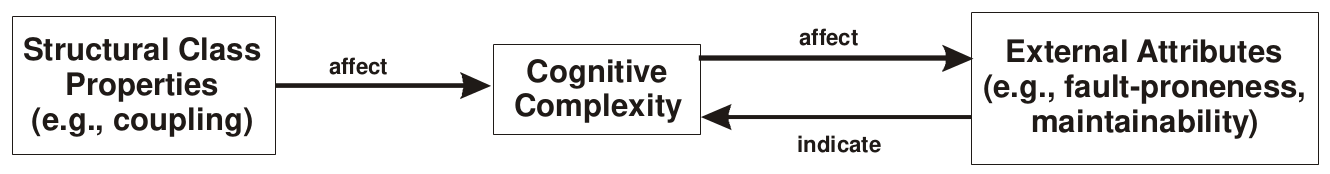
\includegraphics[width=0.5\textwidth]{pictures/faultyclasses1.png}}
	\caption{Theoretical basis for the development of object oriented product metrics \cite{b7radjenovic2013software}.}
	\label{figCoupling}
\end{figure}

\begin{figure}[htbp]
	\centerline{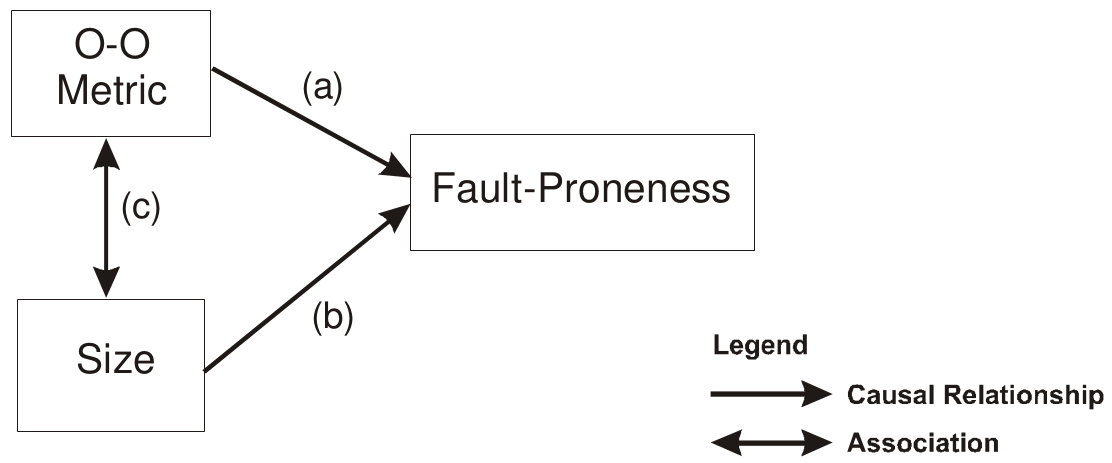
\includegraphics[width=0.45\textwidth]{pictures/faultyclasses2.png}}
	\caption{Path diagram illustrating the confounding effect of class size on the relationship between an object-oriented metric and fault-proneness \cite{b7radjenovic2013software}.}
	\label{figSize}
\end{figure}


\begin{table}
	\caption{Metrics about fault-proneness.}~\label{tab:metrics}
	
	\setlength\tabcolsep{3pt}
	\renewcommand{\arraystretch}{1.4}% for the vertical padding
	\begin{tabularx}{\columnwidth}{ | c | p{5.8cm} || c | }
		\hline
		Abbrevation & Definition & Sources \\ \hline\hline
		LSCC & low-level design class cohesion metric & \cite{b3al2012fault} \\ \hline
		LOC & Lack of Cohesion counts ..  & \cite{b15chidamber1991towards} \\ \hline
		DOI & Depth of Inheritance .. & \cite{b15chidamber1991towards} \\ \hline
		PCCC & path connectivity class cohesion & ... \\ \hline
	\end{tabularx}
\end{table}


\subsection{Method-Method Interaction-Based Cohesion Metrics for Object-Oriented Classes}

Basic units of design in object-oriented programs are classes. Class cohesion refers to the relatedness of class members, i.e., their attributes and methods. Multiple metrics for class cohesion have been proposed in the literature. These object-oriented metrics are based on information available during the high-level or low-level design phases.
In this paper, a formula that accurately measures the degree of interaction between each pair of methods is proposed and used as the basis for introducing a low-level design class cohesion (LSCC) metric \cite{b8al2012precise}. Low-level design (LLD) cohesion metrics use more finely resolved information than that used by High-level design (HLD) cohesion metrics. HLD cohesion metrics identify potential cohesion issues early in the HLD phase. 
In figure \ref{fig1}, rectangles represent methods, circles indicate attributes, and links illustrate the use of attributes by methods of a class. Metrics based on counting the number of links, i.e., the use of attributes by a method, can indicate whether a class is strongly or weakly cohesive. This finely granulated
information is important to help software developers refactoring their code and detecting which methods to possibly remove, i.e., the methods that exhibit even no
links with other methods. When a method-method interaction (MMI) metric
is applied to measure the cohesion for the class shown in figure \ref{fig1}, the
connectivity between each pair of methods is calculated, and it is clearly seen that
method $m_3$ is weakly interconnected to other methods in this class.

\begin{figure}[htbp]
	\centerline{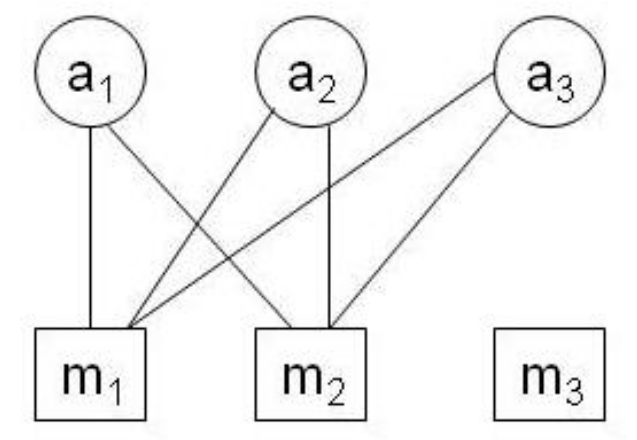
\includegraphics[width=0.2\textwidth]{pictures/am.png}}
	\caption{Sample representative graph for a hypothetical class \cite{b3al2012fault}.}
	\label{fig1}
\end{figure}

As shown in figure \ref{fig2}, there are four other classes with a different method-method interconnection. The class cohesion (CC) of Bonja and Kidanmariam is the ratio of the summation of the similarities between all pairs of methods to the total number of pairs of methods \cite{bonja2006metrics}. The similarity between methods $i$ and $j$ is defined as
\begin{displaymath}
	sim(i,j)=\frac{|I_i \cap I_j|}{|I_i \cup I_j|} ,  
\end{displaymath}
where $I_i$ and $I_j$ are the sets of attributes linked by methods $i$ and $j$, respectivly \cite{b3al2012fault}. In contrast with the class cohesion metric of Pena (SCOM), the calculation is defined as follows
\begin{displaymath}
	sim(i,j)=\frac{|I_i \cap I_j|}{min(|I_i|, |I_j|)} \cdot \frac{|I_i \cup I_j|}{n},  
\end{displaymath}
where $n$ is the number of attributes \cite{fernandez2006sensitive}.
Both CC and SCOM neither consider transitive MMI nor account for inheritance or different method types, and they have not been empirically validated against external quality attributes such as fault occurrences. Of course, there are many other metrics of this kind but the results for the metrics that consider the degree of interaction between each pair of methods are very close to each other \cite{b8al2012precise}.

\begin{figure}[htbp]
	\centerline{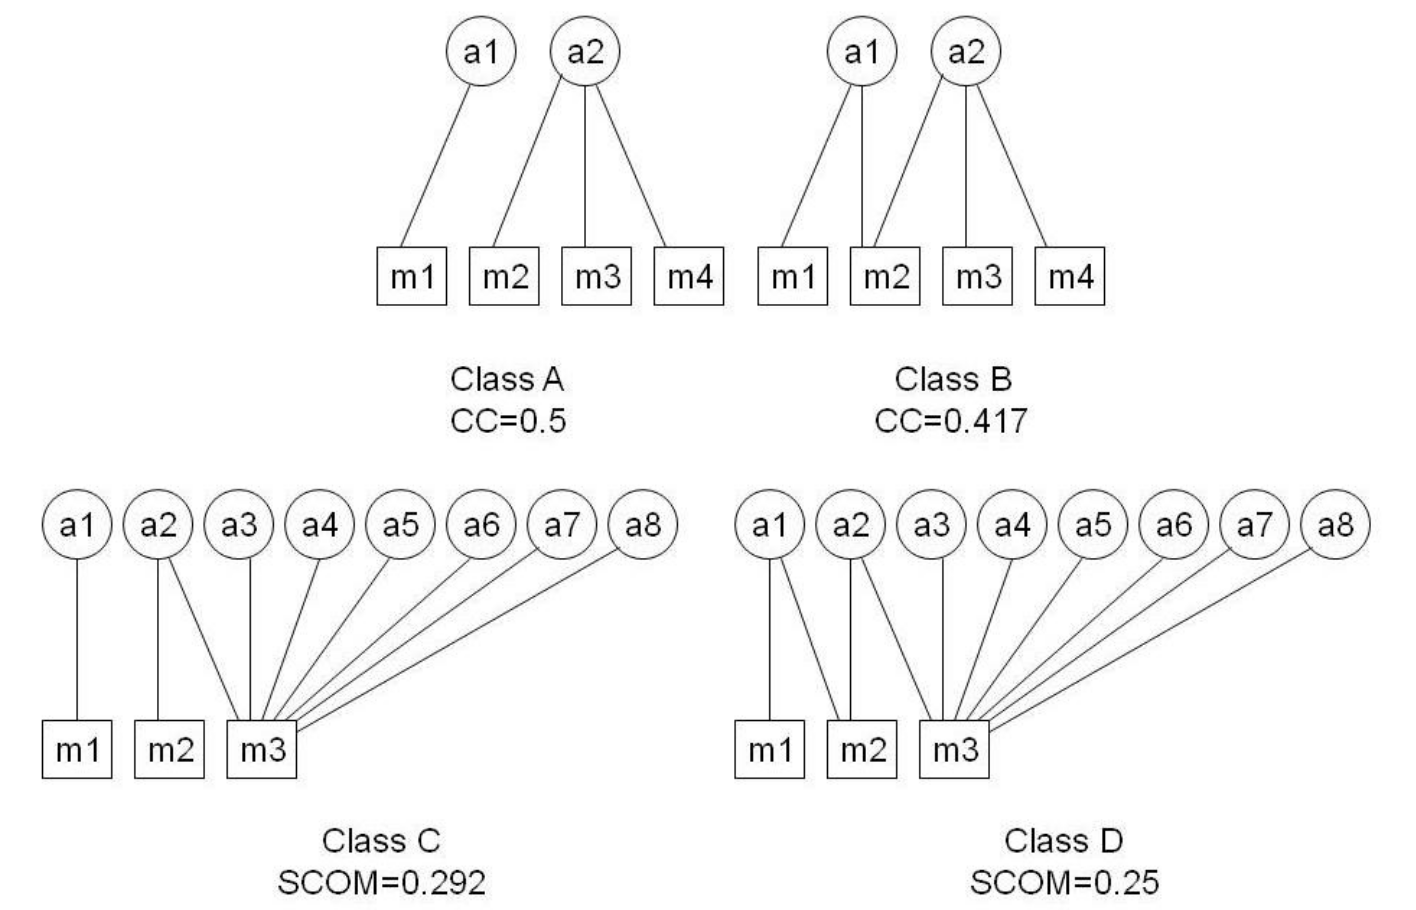
\includegraphics[width=0.4\textwidth]{pictures/am2.png}}
	\caption{Classes with different method-method connectivity patterns \cite{b3al2012fault}.}
	\label{fig2}
\end{figure}

The results suggest that class quality, as measured in terms of fault occurrences, can be more accurately explained by cohesion metrics that account for the degree of interaction between each pair of methods. The fault prediction of interconnection-based object-oriented class cohesion metrics should help the developer to support refactoring during the LLD phase \cite{b8al2012precise}.


\subsection{A Bayesian Network}

The next method to take a closer look at the fault-proneness is a concise representation of a joint probability distribution on a set of statistical variables. Bayesian methods can be used for assessing software fault content and fault proneness. A bayesian network (BN) is encoded as an acyclic graph of nodes and directed edges \cite{b9pai2007empirical}. Assuming that the relationship can be modeled with a general linear model, the structural and numerical specification for the BN is derived. The model can be thought of as a generalization of existing techniques for assessing software quality. The model consists roughly of two parts, first the method produces a probability distribution of the estimated fault content per class in the system and second the conditional probability that a class contains a fault. 
The structure of the model is a BN model whose underlying representation is the generalized linear model. The definition probabilistic network (acyclic graph $G=(V,E)$; A set $S$, of (prior) conditional probability distributions).
Consider a finite set of random variables $X=\{X_1,X_2,....,X_n\}$. It can be defined that a probabilistic network $N=(G,X) over X$ consists of
 \begin{enumerate}
 	\item[-] a directed acyclic graph $G=(V,E)$, $V$ is the set of nodes in the graph and there is a one-one correspondence between $V$ and $X$. $E \subseteq V \times V$ the set of directed edges, representing conditional independence assumptions, i.e., for each $X_i \in X$, $i(X_i,N D_{x_i}| Pa_{x_i})$ and $N D_{x_i} = X \backslash ({X_i} \cup Des_{x_i})$ 
 	\item[-] a set of (prior) conditional probability distributions, that specifies $p(X_i)| p(Pa_{x_i})$ for each $X_i \in X$, where $Pa_{x_i}$ represents the set of immediate parents of $X$.
 \end{enumerate} 

Once a network is specified over a set of random variables, their marginal and joint probabilities can be computed.
Given a BN structure, the joint probability distribution over $X$ is encoded as

\begin{displaymath}
	p(X)= \prod_{i=1}^{n}p(X_i|P_{ax_i})
\end{displaymath}

And given this joint probability, the marginal probability of a random variable $X_i$ is computed as 

\begin{displaymath}
	p(X_i)= \sum_{X_i,j\neq i}^{n}p(X)
\end{displaymath}

The model parameters that are used are listed in the following \cite{b9pai2007empirical}: 

\begin{itemize}
	\item[1.] Weighted methods per class (\textbf{WMC}): The number of methods implemented in a given class.
	\item[2.] Depth of inheritance tree (\textbf{DOI})
	\item[3.] Response for class (\textbf{RFC}): Number of methods implemented within a class plus the number of methods accessible to an object class due to inheritance. (Traditionally, it represents the number of methods that an object of a given class can execute in response to a received message \cite{b9pai2007empirical}.)
	\item[4.] Number of children (\textbf{NOC}): The number of classes that directly inherit from a given class.
	\item[5.] Coupling between object classes (\textbf{CBO}): The number of distinct non-inheritance related classes to which a given class is coupled. (i.e., when a given class uses the methods or attributes of the coupled class \cite{b9pai2007empirical}.)
	\item[6.] Lack of cohesion in methods (\textbf{LCOM}): A measure of the degree to which a class represents single or multiple abstractions. There are varying definitions for LCOM. (i.e., by computing the average percentage of methods in a given class using each attribute of that class, and then subtracting that percentage from 100 percent \cite{b9pai2007empirical}.)
	\item[7.] Source lines of code (\textbf{SLOC}): This is measured as the total lines of source code in the class and serves as a measure of class size.
\end{itemize}

The dependent variables, which serve as surrogate metrics of software quality, are
\begin{itemize}
	\item Fault Content (FC): We define fault content as the number of faults per class. The estimation of ourmodel is a (marginal) conditional probability ofobserving a certain number of faults per class, giventhe metrics for that class.
	\item Fault proneness (FP): The conditional probability thata class contains a fault, given the metrics for that class.
\end{itemize}

\begin{figure}[htbp]
	\centerline{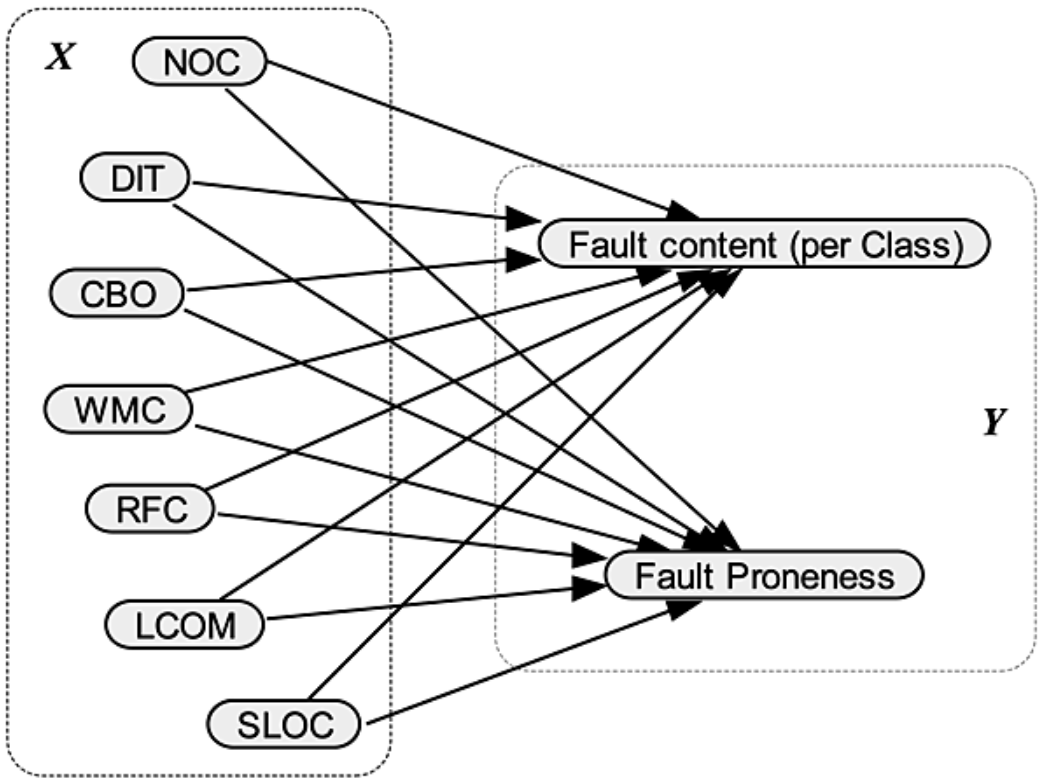
\includegraphics[width=0.4\textwidth]{pictures/bn2.png}}
	\caption{BN model for fault content and fault-proneness analysis.}
	\label{fig2bn}
\end{figure}

The model construction is as follows

\begin{figure}[htbp]
	\centerline{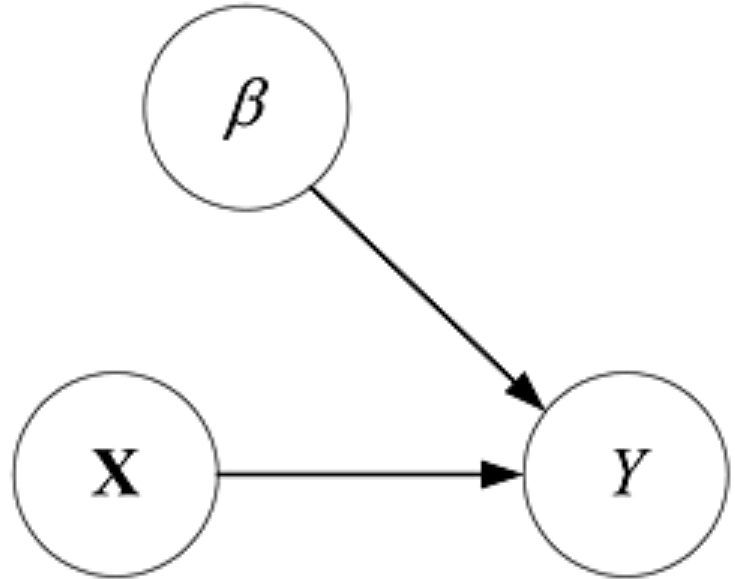
\includegraphics[width=0.2\textwidth]{pictures/bn1.png}}
	\caption{BN representation of a general linear model.}
	\label{fig1bn}
\end{figure}


The results also show that this model producesthese estimations at a statistically significant level.

- RESULTS 

- BN: the results of performing multiple regression, the metrics WMC, CBO, RFC, and SLOC are very significant for assessing both fault content and fault proneness

- this specific set of predictors is very significant for assessing fault content and fault proneness in large software systems

- it was observed that import coupling (that count the number of other classes called by a class) metrics are strongly associated with fault
pron and predict faulty classes with high accuracy

- Associate refactoring to the last sections

\section{Discussion}

The Class Buffer model is more scalable over the three facets compared to other frameworks for viewing large scale data: data size, perceptual processing, and computation speed.
The enhanced perceptual processing arises from the broad spectrum of visualization methods that can be generated for density maps of multiple classes.
The model on the other hand does not guide users in a very good way. The challenges of understanding and using the different visualization methods have to be further investigated.
Multiclass density maps often have the disadvantage of obfuscating information when mixing or masking is introduced but they can also display more data classes that can be easily shown when using dot density maps. Different classes intersect, overlap and interfere with each other and by this make it hard to understand these kind of maps.
There are a multitude of visualization results that appear to visualize the data in a reasonably good way, but often the results obfuscate the data in a way that makes it hard to comprehend the full scope of the information present. In example the data that gets presented often mix or mask certain areas of interest. This results in clusters being mixed with neighboring clusters and thus losing the possibility to show the true amount of datapoints present in one group. Additionally outliers get overlaid by datapoints from other groups or get scaled down to an extend that they cannot be perceived at all when using the visualization methods provided by the Class Buffer model implementation, this effect can be seen in Figure~\ref{fig:outliers}.

\begin{figure}
	\centering
	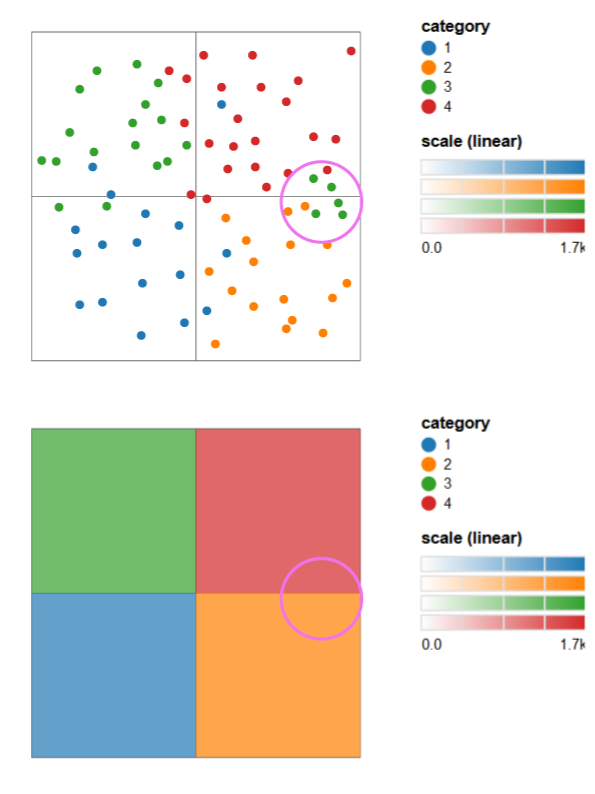
\includegraphics[width=0.85\columnwidth]{./figures/outliers}
	\caption[outliers]{A portrayal of the effect present when masking classes with other classes. In the top picture the data is visualized as a standard 2D scatterplot. The group of outliers get lost in the visualization process, which can be seen in the bottom picture.}~\label{fig:outliers}
\end{figure}

The Class Buffer model implemented by Jo et al. uses different approaches to display data but just few of them result in classical density maps~\cite{jo2019declarative}, some also arouse the impression of dot density maps with different tiling or aggregation.
A density map can be more challenging to comprehend when used in the wrong context or when implemented wrong or without an appropriate understanding of the field.\\It is thus essential to improve the presented method further. This could be done by enhancing the visual separation with additional options or by implementing an expressive guiding toolbox or some other kind of guideline. By providing the user with the basic tools to generate multiclass density maps the first step has been taken.

% \textcolor{red}{\lipsum[1]}

% \improvement{Clusters are seperable, outliers get lost}

\section{Conclusion}\label{conclusion}

In the future, as well as today, fault-proneness estimation and prediction could play a key role in software product quality control.  In this area, much effort has been invested in defining metrics and identifying models for system evaluation, object-oriented models as well as others.  Using these metrics to assess which parts of the system are more fault-proneness is of primary importance, as summarized in this paper.
Much work has concentrated on how to select the software metrics that are most likely to indicate fault-proneness. 

In the field of software evolution, metrics can be used for identifying stable or unstable parts of software systems.

Moreover the question is, what can really prevent faults in the later used system beforehand?

If you take up the other software trends of development mentioned at the beginning, it becomes clear that they are all connected in a certain way. The fault-proneness and the maintenance grow with increasing complexity.Ensuring security and quality always involves a number of features.

%- summarize discussion and results; name important metrics/properties that should stay in mind after reading this

%- what can reduce the fault-pron in software development

%- outlook future work (future work wäre größere systeme anschauen und testen auf faulty classes und metriken testen an sich)

%- This paper discussed the concept of fault proneness using the example of object-oriented programming and design metrics, which means that for the most part the results can only be transferred to the object-oriented context.


%- final catch and the link to the superordinate context (research trends in software technology); link to introduction and motivation

%wie in related work aufgezeigt die flexible metrics die können als ausblick hilfreich sien wenn sich der kontexxt leicht ändert

%\begin{abstract}
	This document is a model and instructions for \LaTeX.
	This and the IEEEtran.cls file define the components of your paper [title, text, heads, etc.]. *CRITICAL: Do Not Use Symbols, Special Characters, Footnotes, 
	or Math in Paper Title or Abstract.
\end{abstract}

\section{Ease of Use}

\subsection{Maintaining the Integrity of the Specifications}

The IEEEtran class file is used to format your paper and style the text. All margins, 
column widths, line spaces, and text fonts are prescribed; please do not 
alter them. You may note peculiarities. For example, the head margin
measures proportionately more than is customary. This measurement 
and others are deliberate, using specifications that anticipate your paper 
as one part of the entire proceedings, and not as an independent document. 
Please do not revise any of the current designations.

\section{Prepare Your Paper Before Styling}
Before you begin to format your paper, first write and save the content as a 
separate text file. Complete all content and organizational editing before 
formatting. Please note sections \ref{AA}--\ref{SCM} below for more information on 
proofreading, spelling and grammar.

Keep your text and graphic files separate until after the text has been 
formatted and styled. Do not number text heads---{\LaTeX} will do that 
for you.

\subsection{Abbreviations and Acronyms}\label{AA}
Define abbreviations and acronyms the first time they are used in the text, 
even after they have been defined in the abstract. Abbreviations such as 
IEEE, SI, MKS, CGS, ac, dc, and rms do not have to be defined. Do not use 
abbreviations in the title or heads unless they are unavoidable.

\subsection{Units}
\begin{itemize}
	\item Use either SI (MKS) or CGS as primary units. (SI units are encouraged.) English units may be used as secondary units (in parentheses). An exception would be the use of English units as identifiers in trade, such as ``3.5-inch disk drive''.
	\item Avoid combining SI and CGS units, such as current in amperes and magnetic field in oersteds. This often leads to confusion because equations do not balance dimensionally. If you must use mixed units, clearly state the units for each quantity that you use in an equation.
	\item Do not mix complete spellings and abbreviations of units: ``Wb/m\textsuperscript{2}'' or ``webers per square meter'', not ``webers/m\textsuperscript{2}''. Spell out units when they appear in text: ``. . . a few henries'', not ``. . . a few H''.
	\item Use a zero before decimal points: ``0.25'', not ``.25''. Use ``cm\textsuperscript{3}'', not ``cc''.)
\end{itemize}

\subsection{Equations}
Number equations consecutively. To make your 
equations more compact, you may use the solidus (~/~), the exp function, or 
appropriate exponents. Italicize Roman symbols for quantities and variables, 
but not Greek symbols. Use a long dash rather than a hyphen for a minus 
sign. Punctuate equations with commas or periods when they are part of a 
sentence, as in:
\begin{equation}
	a+b=\gamma\label{eq}
\end{equation}

Be sure that the 
symbols in your equation have been defined before or immediately following 
the equation. Use ``\eqref{eq}'', not ``Eq.~\eqref{eq}'' or ``equation \eqref{eq}'', except at 
the beginning of a sentence: ``Equation \eqref{eq} is . . .''

\subsection{\LaTeX-Specific Advice}

Please use ``soft'' (e.g., \verb|\eqref{Eq}|) cross references instead
of ``hard'' references (e.g., \verb|(1)|). That will make it possible
to combine sections, add equations, or change the order of figures or
citations without having to go through the file line by line.

Please don't use the \verb|{eqnarray}| equation environment. Use
\verb|{align}| or \verb|{IEEEeqnarray}| instead. The \verb|{eqnarray}|
environment leaves unsightly spaces around relation symbols.

Please note that the \verb|{subequations}| environment in {\LaTeX}
will increment the main equation counter even when there are no
equation numbers displayed. If you forget that, you might write an
article in which the equation numbers skip from (17) to (20), causing
the copy editors to wonder if you've discovered a new method of
counting.

{\BibTeX} does not work by magic. It doesn't get the bibliographic
data from thin air but from .bib files. If you use {\BibTeX} to produce a
bibliography you must send the .bib files. 

{\LaTeX} can't read your mind. If you assign the same label to a
subsubsection and a table, you might find that Table I has been cross
referenced as Table IV-B3. 

{\LaTeX} does not have precognitive abilities. If you put a
\verb|\label| command before the command that updates the counter it's
supposed to be using, the label will pick up the last counter to be
cross referenced instead. In particular, a \verb|\label| command
should not go before the caption of a figure or a table.

Do not use \verb|\nonumber| inside the \verb|{array}| environment. It
will not stop equation numbers inside \verb|{array}| (there won't be
any anyway) and it might stop a wanted equation number in the
surrounding equation.

\subsection{Some Common Mistakes}\label{SCM}
\begin{itemize}
	\item The word ``data'' is plural, not singular.
	\item The subscript for the permeability of vacuum $\mu_{0}$, and other common scientific constants, is zero with subscript formatting, not a lowercase letter ``o''.
	\item In American English, commas, semicolons, periods, question and exclamation marks are located within quotation marks only when a complete thought or name is cited, such as a title or full quotation. When quotation marks are used, instead of a bold or italic typeface, to highlight a word or phrase, punctuation should appear outside of the quotation marks. A parenthetical phrase or statement at the end of a sentence is punctuated outside of the closing parenthesis (like this). (A parenthetical sentence is punctuated within the parentheses.)
	\item A graph within a graph is an ``inset'', not an ``insert''. The word alternatively is preferred to the word ``alternately'' (unless you really mean something that alternates).
	\item Do not use the word ``essentially'' to mean ``approximately'' or ``effectively''.
	\item In your paper title, if the words ``that uses'' can accurately replace the word ``using'', capitalize the ``u''; if not, keep using lower-cased.
	\item Be aware of the different meanings of the homophones ``affect'' and ``effect'', ``complement'' and ``compliment'', ``discreet'' and ``discrete'', ``principal'' and ``principle''.
	\item Do not confuse ``imply'' and ``infer''.
	\item The prefix ``non'' is not a word; it should be joined to the word it modifies, usually without a hyphen.
	\item There is no period after the ``et'' in the Latin abbreviation ``et al.''.
	\item The abbreviation ``i.e.'' means ``that is'', and the abbreviation ``e.g.'' means ``for example''.
\end{itemize}
An excellent style manual for science writers is \cite{b7}.

\subsection{Authors and Affiliations}
\textbf{The class file is designed for, but not limited to, six authors.} A 
minimum of one author is required for all conference articles. Author names 
should be listed starting from left to right and then moving down to the 
next line. This is the author sequence that will be used in future citations 
and by indexing services. Names should not be listed in columns nor group by 
affiliation. Please keep your affiliations as succinct as possible (for 
example, do not differentiate among departments of the same organization).

\subsection{Identify the Headings}
Headings, or heads, are organizational devices that guide the reader through 
your paper. There are two types: component heads and text heads.

Component heads identify the different components of your paper and are not 
topically subordinate to each other. Examples include Acknowledgments and 
References and, for these, the correct style to use is ``Heading 5''. Use 
``figure caption'' for your Figure captions, and ``table head'' for your 
table title. Run-in heads, such as ``Abstract'', will require you to apply a 
style (in this case, italic) in addition to the style provided by the drop 
down menu to differentiate the head from the text.

Text heads organize the topics on a relational, hierarchical basis. For 
example, the paper title is the primary text head because all subsequent 
material relates and elaborates on this one topic. If there are two or more 
sub-topics, the next level head (uppercase Roman numerals) should be used 
and, conversely, if there are not at least two sub-topics, then no subheads 
should be introduced.

\subsection{Figures and Tables}
\paragraph{Positioning Figures and Tables} Place figures and tables at the top and 
bottom of columns. Avoid placing them in the middle of columns. Large 
figures and tables may span across both columns. Figure captions should be 
below the figures; table heads should appear above the tables. Insert 
figures and tables after they are cited in the text. Use the abbreviation 
``Fig.~\ref{fig}'', even at the beginning of a sentence.

\begin{table}[htbp]
	\caption{Table Type Styles}
	\begin{center}
		\begin{tabular}{|c|c|c|c|}
			\hline
			\textbf{Table}&\multicolumn{3}{|c|}{\textbf{Table Column Head}} \\
			\cline{2-4} 
			\textbf{Head} & \textbf{\textit{Table column subhead}}& \textbf{\textit{Subhead}}& \textbf{\textit{Subhead}} \\
			\hline
			copy& More table copy$^{\mathrm{a}}$& &  \\
			\hline
			\multicolumn{4}{l}{$^{\mathrm{a}}$Sample of a Table footnote.}
		\end{tabular}
		\label{tab1}
	\end{center}
\end{table}

\begin{figure}[htbp]
	\centerline{\includegraphics{fig1.png}}
	\caption{Example of a figure caption.}
	\label{fig}
\end{figure}

Figure Labels: Use 8 point Times New Roman for Figure labels. Use words 
rather than symbols or abbreviations when writing Figure axis labels to 
avoid confusing the reader. As an example, write the quantity 
``Magnetization'', or ``Magnetization, M'', not just ``M''. If including 
units in the label, present them within parentheses. Do not label axes only 
with units. In the example, write ``Magnetization (A/m)'' or ``Magnetization 
\{A[m(1)]\}'', not just ``A/m''. Do not label axes with a ratio of 
quantities and units. For example, write ``Temperature (K)'', not 
``Temperature/K''.

\section*{Acknowledgment}

The preferred spelling of the word ``acknowledgment'' in America is without 
an ``e'' after the ``g''. Avoid the stilted expression ``one of us (R. B. 
G.) thanks $\ldots$''. Instead, try ``R. B. G. thanks$\ldots$''. Put sponsor 
acknowledgments in the unnumbered footnote on the first page.

%\begin{IEEEkeywords}
%component, formatting, style, styling, insert
%\end{IEEEkeywords}

%\color{red}
IEEE conference templates contain guidance text for composing and formatting conference papers. Please ensure that all template text is removed from your conference paper prior to submission to the conference. Failure to remove the template text from your paper may result in your paper not being published.

\section*{References}

Please number citations consecutively within brackets \cite{b1}. The 
sentence punctuation follows the bracket \cite{b2}. Refer simply to the reference 
number, as in \cite{b3}---do not use ``Ref. \cite{b3}'' or ``reference \cite{b3}'' except at 
the beginning of a sentence: ``Reference \cite{b3} was the first $\ldots$''

Number footnotes separately in superscripts. Place the actual footnote at 
the bottom of the column in which it was cited. Do not put footnotes in the 
abstract or reference list. Use letters for table footnotes.

Unless there are six authors or more give all authors' names; do not use 
``et al.''. Papers that have not been published, even if they have been 
submitted for publication, should be cited as ``unpublished'' \cite{b4}. Papers 
that have been accepted for publication should be cited as ``in press'' \cite{b5}. 
Capitalize only the first word in a paper title, except for proper nouns and 
element symbols.

For papers published in translation journals, please give the English 
citation first, followed by the original foreign-language citation \cite{b6}.

\begin{thebibliography}{00}
	\bibitem{ba1} G. Eason, B. Noble, and I. N. Sneddon, ``On certain integrals of Lipschitz-Hankel type involving products of Bessel functions,'' Phil. Trans. Roy. Soc. London, vol. A247, pp. 529--551, April 1955.
	\bibitem{ba2} J. Clerk Maxwell, A Treatise on Electricity and Magnetism, 3rd ed., vol. 2. Oxford: Clarendon, 1892, pp.68--73.
	\bibitem{ba3} I. S. Jacobs and C. P. Bean, ``Fine particles, thin films and exchange anisotropy,'' in Magnetism, vol. III, G. T. Rado and H. Suhl, Eds. New York: Academic, 1963, pp. 271--350.
	\bibitem{ba4} K. Elissa, ``Title of paper if known,'' unpublished.
	\bibitem{ba5} R. Nicole, ``Title of paper with only first word capitalized,'' J. Name Stand. Abbrev., in press.
	\bibitem{ba6} Y. Yorozu, M. Hirano, K. Oka, and Y. Tagawa, ``Electron spectroscopy studies on magneto-optical media and plastic substrate interface,'' IEEE Transl. J. Magn. Japan, vol. 2, pp. 740--741, August 1987 [Digests 9th Annual Conf. Magnetics Japan, p. 301, 1982].
	\bibitem{ba7} M. Young, The Technical Writer's Handbook. Mill Valley, CA: University Science, 1989.
\end{thebibliography}

\bibliographystyle{IEEEtran}
\bibliography{masterseminar}

\end{document}
